\documentclass[sigconf]{acmart}
\usepackage{geometry}
\geometry{a4paper, margin=1in}
\bibliographystyle{plain}
\usepackage{graphicx}
\usepackage{hyperref}
\usepackage{listings}
\usepackage{xcolor}
\usepackage{float}

\definecolor{codegreen}{rgb}{0,0.6,0}
\definecolor{codegray}{rgb}{0.5,0.5,0.5}
\definecolor{codepurple}{rgb}{0.58,0,0.82}
\definecolor{backcolour}{rgb}{0.95,0.95,0.92}

\lstdefinestyle{mystyle}{
    backgroundcolor=\color{backcolour},   
    commentstyle=\color{codegreen},
    keywordstyle=\color{magenta},
    numberstyle=\tiny\color{codegray},
    stringstyle=\color{codepurple},
    basicstyle=\ttfamily\footnotesize,
    breakatwhitespace=false,         
    breaklines=true,                 
    captionpos=b,                    
    keepspaces=true,                 
    numbers=left,                    
    numbersep=5pt,                  
    showspaces=false,                
    showstringspaces=false,
    showtabs=false,                  
    tabsize=2
}

\lstset{style=mystyle}

\begin{document}

\title{Quality Assignment Report}
\subtitle{\\[0.5cm] Advanced Software Quality and Security 2025 \\ Software Quality \\ Instructor: Dr. Matteo Esposito \\ University of Oulu}

\author{Walter Määttä}
\affiliation{%
  \institution{University of Oulu}
  \city{Oulu}
  \country{Finland}
}

\author{Väinö-Ilmari Kasurinen}
\affiliation{%
  \institution{University of Oulu}
  \city{Oulu}
  \country{Finland}
}

\author{Juuso Anttila}
\affiliation{%
  \institution{University of Oulu}
  \city{Oulu}
  \country{Finland}
}

\author{Niko Siltala}
\affiliation{%
  \institution{University of Oulu}
  \city{Oulu}
  \country{Finland}
}

\date{\today}


% Abstract
\begin{abstract}
This report presents a comprehensive quality assessment of the LLM Message Dispatch Tool project, a system designed to facilitate communication with various LLM implementations. The assessment includes an architectural review, test plan documentation, detailed analysis of LLM integration, and software quality evaluation using industry tools like SonarQube and CodeScene. The report also incorporates findings from LLM-assisted code analysis to provide insights into both our student project and the open-source Apache Kafka project. Key findings include several security vulnerabilities in container configuration and protocol usage, code quality issues related to duplication and maintainability, and architectural considerations for improving system robustness. The report concludes with prioritized implementation recommendations to address the identified issues.
\end{abstract}

\maketitle

% 1 Intro
\section{Introduction}
Modern software engineering practices emphasize the importance of quality assurance throughout the development lifecycle. With the increasing prominence of Large Language Models (LLMs) in software applications, ensuring the quality and security of systems that integrate with these models has become particularly important. This report examines the quality aspects of the LLM Message Dispatch Tool, a system designed to facilitate communication between users and various LLM implementations.

The LLM Message Dispatch Tool is built using a modern architecture with a FastAPI backend, React frontend, and MongoDB database. It allows users to compose and send messages to different LLM services, store responses, and review previous interactions. The system's architecture includes components for message handling, LLM integration, and data persistence, making it a representative example of contemporary full-stack development with AI integration.

Our quality assessment covers multiple dimensions, including architectural design, testing methodology, LLM integration techniques, code quality metrics, and security vulnerabilities. We employed industry-standard tools such as SonarQube and CodeScene for automated analysis, supplemented by LLM-assisted code review to identify potential improvements. By combining these approaches, we aim to provide a holistic view of the system's quality attributes and actionable recommendations for enhancement.

% 2 Methods
\section{Methodology}
Our quality assessment methodology incorporated multiple complementary approaches to gain a comprehensive understanding of the system's quality attributes:

\subsection{Architectural Analysis}
We examined the system's architecture through UML diagrams representing both backend and frontend components (see Figures \ref{fig:figure1} and \ref{fig:figure2}). The analysis focused on identifying key components, their interactions, and potential architectural weaknesses such as tight coupling, insufficient abstraction, and scalability limitations.

\begin{figure}[htbp]
    \centering
    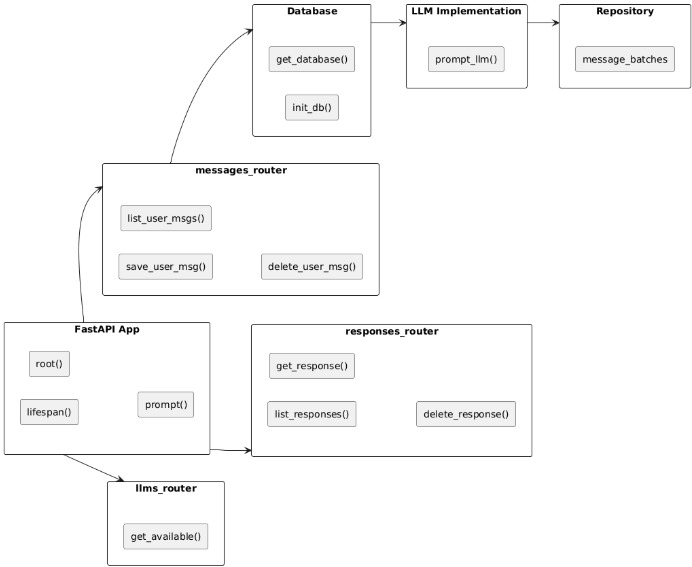
\includegraphics[width=1\linewidth]{BackUML.jpg}
    \caption{Backend UML Diagram}
    \label{fig:figure1}
\end{figure}

\begin{figure}[htbp]
    \centering
    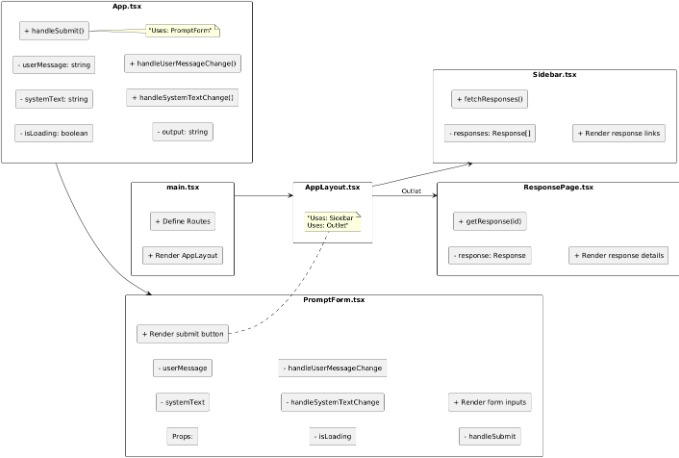
\includegraphics[width=1\linewidth]{FrontUML.jpg}
    \caption{Frontend UML Diagram}
    \label{fig:figure2}
\end{figure}

\subsection{Test Planning and Documentation}
We developed a test plan covering various aspects of the system (see test\_plan.pdf), including API routes, database connections, LLM integration, and error handling. The test plan included unit tests, integration tests, performance tests, and robustness tests, with detailed test cases and expected outcomes.

\subsection{LLM Integration Assessment}
We analyzed the implementation of LLM integration, including RAG (Retrieval-Augmented Generation) techniques, embeddings, and prompt engineering. This included examining how the system loads and processes source code for analysis, chunking strategies, and system prompts used for interactions with the language model.

\subsection{Automated Quality Analysis}
We utilized industry-standard tools including SonarQube and CodeScene to perform automated analysis of code quality. These tools provided metrics and identified issues related to security vulnerabilities, code duplication, maintainability problems, and other quality concerns.

\subsection{LLM-Assisted Code Analysis}
We employed LLM-assisted analysis to examine both our student project and selected components of the Apache Kafka open-source project. This analysis involved loading source code into a FAISS vectorstore for RAG enrichment and using a specialized system prompt to guide the language model's analysis of code quality.

\subsection{Comparative Analysis}
We compared and synthesized findings from the various analysis methods to identify common patterns, prioritize issues, and develop actionable recommendations. This comparative approach helped ensure that our conclusions were robust and supported by multiple lines of evidence.

% 3 Results and Discussion
\section{Results and Discussion}

\subsection{Detailed report on LLM integration, including fine-tuning, embeddings, RAG, and prompt engineering}
For the RAG-analysis of our project, we loaded the source code of the LLM Message Dispatch tool backend for analysis. It was loaded into a FAISS vectorstore for RAG-enrichment. The documents were separated into chunks of 500 with an overlap of 100 to preserve appropriate context. With a default context size of 2048 we decided on 5 documents so that the model can fetch enough relevant files for the analysis, which is especially important when different software modules are imported.

For the RAG, we used HuggingFace's embeddings with sentence-transformers/all-mpnet-base-v2 as the model and the embedding creation was accelerated with the GPU for faster processing.

For the analysis, we specified a system message to the LLM:
"You are an assistant in code quality analysis.
You need to look for source code quality improvements.
Suggest a remediation for the identified issue.
DO NOT HALLUCINATE.
Source code:
\{code\}"

This system message gives important context to the model and specifies its goal. The DO NOT HALLUCINATE line has been found to reduce the chances of hallucination since the model has higher chance to self-reflect its output. Additionally, the source code of the analyzed class is of course provided as a part of the prompt in the input variable.

For the LLM Message Dispatch Tool backend itself we did not use RAG. The application supports any model that the host machine has through ollama. We found the default parameters, such as the temperature and context size appropriate for the use case. Furthermore, as the point of the application is for the user to provide the system message in conjunction with the user message, we did not give the model any unnecessary information that could decrease the model performance from the user's experience.

\subsection{Backend Overview}
The backend is built using the FastAPI framework and provides REST API endpoints that allow for managing messages, LLM templates, and responses. The backend uses MongoDB as a database and includes the following features:

API endpoints:
\begin{itemize}
\item Store, retrieve, and delete messages.
\item Select and manage LLM templates.
\item Send prompts and store responses.
\end{itemize}

Database connection:
\begin{itemize}
\item MongoDB connection is centrally initialized and managed.
\end{itemize}

Docker support:
\begin{itemize}
\item The backend can be launched using Docker, making development and deployment easier.
\end{itemize}

\subsection{Frontend Overview}
The frontend of this project is a React application built with TypeScript and uses Vite as the build tool. It is designed to provide a user-friendly interface for interacting with the backend API. The application is structured to ensure modularity, scalability, and maintainability, with reusable components and a clear separation of concerns.

Key Features:
\begin{itemize}
\item The application is divided into reusable components, such as AppLayout, Sidebar, PromptForm, and DropdownMenu, which handle specific parts of the UI. This modular approach makes the codebase easier to maintain and extend.
\item The application uses React Router for client-side routing. The key routes include / to display the main application interface and /responses/:id to display detailed information about a specific response.
\item Tailwind CSS is used for styling, ensuring a modern and responsive design. Global styles are defined in App.css and index.css.
\item Local state is managed using React's useState and useEffect hooks. Components like PromptForm and Sidebar fetch and manage data dynamically from the backend.
\item The frontend communicates with the backend API to fetch and display data such as available LLMs, user messages, and system responses. API calls are made using the fetch API, and error handling is implemented to ensure robustness.
\item The application is thoroughly tested using Vitest and React Testing Library. Tests cover key components and user interactions, ensuring reliability and preventing regressions.
\item The project includes a code coverage report generated by Istanbul. The current test coverage is over 90\%, demonstrating a strong focus on quality assurance.
\end{itemize}

\section{Software quality evaluation results from SonarQube and CodeScene}
\subsection{Sonarqube}
You can find the raw results at sonarqube\_issues.xlsx.

\subsection{Codescene}
You can find the results at codescene.pdf.

\section{LLM-assisted analysis findings for both the student and the open-source projects}
\subsection{Our project – LLM Message Dispatch Tool}
You can find the raw analysis result in the rag\_analysis.md file.

\subsection{Apache Kafka analysis}
You can find the analysis results from 20 different classes of the Apache Kafka project from the kafka\_analysis.md file.

\section{A comparative summary of insights from SonarQube, CodeScene, and the LLM}
\subsection{Critical Security Vulnerabilities}
The first security weakness revealed by the analysis is the running of the privileged containers (docker-S6471). As can be seen from Figure \ref{fig:figure3}, the "python" Docker is running with the default "root" privileges. The default configuration is risky because the containers can be vulnerable to break-out attacks, thus compromising the host system. When processes run with root privileges, the processes run with full access across the container, meaning any vulnerability exploited from the application would result in the elevation of root privileges. The security scan tools rate this weakness as medium priority. To mitigate this weakness, the creation of a specific user with limited privileges in the Dockerfile would greatly minimize the possible attack surface. This practice aligns with broadly accepted security best practices since it follows the principle of least privilege in container configuration. Additionally, when applications are deployed on orchestration platforms like Kubernetes, the use of appropriate security context configurations would provide additional layers of security.

\begin{figure}[htbp]
    \centering
    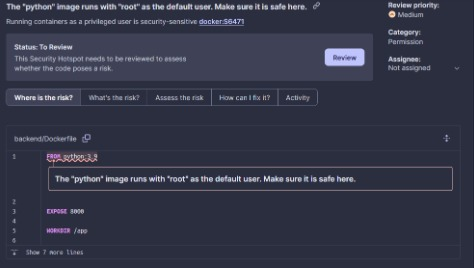
\includegraphics[width=1\linewidth]{Image1.jpg}
    \caption{Python Docker container running with root privileges.}
    \label{fig:figure3}
\end{figure}

The other serious security issue highlighted in Figure \ref{fig:figure4} is the risky practice of file duplication (docker-S6470). The Dockerfile is a prime example of unnecessary copying of context directories, which can inadvertently leak sensitive information held within the container. Inadvertently, such practices may involve the inclusion of hidden files like .env, .git, or credential files with the final product. API keys, database credentials, or other sensitive information being exposed poses a serious security threat. In addition, the practice leads to the generation of large Docker images with unnecessary content, thus increasing the attack surface. The unparameterized COPY commands used with no exclusions deserve special attention.

\begin{figure}[htbp]
    \centering
    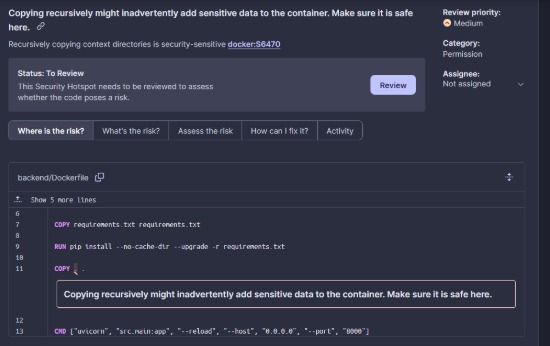
\includegraphics[width=1\linewidth]{Image2.jpg}
    \caption{Risky file duplication in Dockerfile.}
    \label{fig:figure4}
\end{figure}

The use of a comprehensive .dockerignore file would help mitigate this risk by explicitly excluding sensitive files and directories from the build context. In addition, specifying only the necessary files and directories in COPY directives provides another layer of protection. Finally, multi-stage builds offer another method for reducing the ultimate image size and minimizing the potential exposure of sensitive data. In terms of credential management, the use of a dedicated secrets management solution is best practice.

The third security weakness found is shown in Figure \ref{fig:figure5} the use of an unencrypted HTTP protocol in the codebase (python-S5332). Even though this issue is ranked with low severity, it is of significant security risk since data transmission in plain text is vulnerable to man-in-the-middle attacks. Authentication credentials transmitted over HTTP are vulnerable to interception, and without encryption mechanisms, the content's integrity cannot be guaranteed. Shifting all external communications to HTTPS would practically eliminate this vulnerability. This change should be complemented with the correct protocols for certificate checks to prevent attacks based on certificates. Configuration arguments, like endpoints, should be managed using environment variables rather than hard-coded values, making deployments easier across varied environments. Further, the usage of TLS/SSL termination for hosted services would go a long way toward making the security framework stronger.

\begin{figure}[htbp]
    \centering
    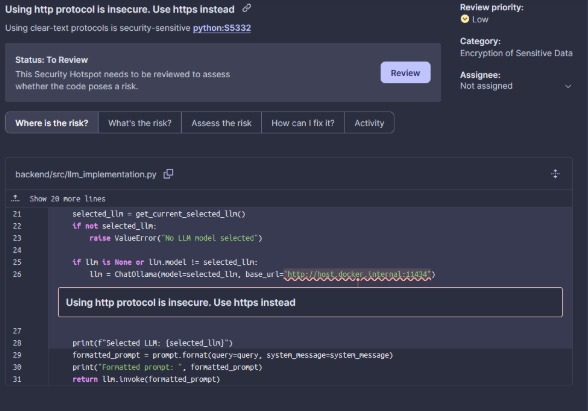
\includegraphics[width=1\linewidth]{Image3.jpg}
    \caption{Unencrypted HTTP protocol in the codebase.}
    \label{fig:figure5}
\end{figure}

\subsection{Code Quality Issues}
Apart from security issues, the codebase has significant code quality concerns. Figure \ref{fig:figure6} displays a high degree of code duplication where four functions in the module—get\allowbreak\_user\allowbreak\_message\allowbreak, get\allowbreak\_system\allowbreak\_message\allowbreak, delete\allowbreak\_user\allowbreak\_message\allowbreak, and delete\allowbreak\_system\allowbreak\_message\allowbreak—share a similar pattern. This pattern violates the Don't Repeat Yourself principle, thereby making maintenance harder because of the need to duplicate changes across different functions. The redundancy increases the chances of inconsistency when changes are applied in one place but not in others. Further, having duplicated code reduces readability for incoming developers who are new to the project.

\begin{figure}[htbp]
    \centering
    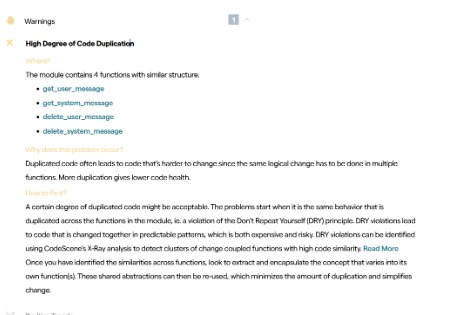
\includegraphics[width=1\linewidth]{Image7.jpg}
    \caption{Code duplication in the module.}
    \label{fig:figure6}
\end{figure}

Solving this problem would require factoring common functionalities into root functions with appropriate parameters. Architectural patterns like the Strategy design or the Template Method can provide high-level solutions for avoiding this redundancy. Creating a message service class responsible for handling user and system messages with a common logical mechanism would considerably improve the maintainability of the application and lower the chance of inconsistencies. Figures \ref{fig:figure7} and \ref{fig:figure8} demonstrate additional maintainability issues within the codebase include commented-out code that should be removed entirely, unnecessary type assertions that add complexity without any benefits, components lacking proper read-only specifiers, and accessibility issues regarding form labels. The frontend architecture shows components that are highly coupled, which would benefit from refactoring to make them more maintainable in the long run.

\begin{figure}[htbp]
    \centering
    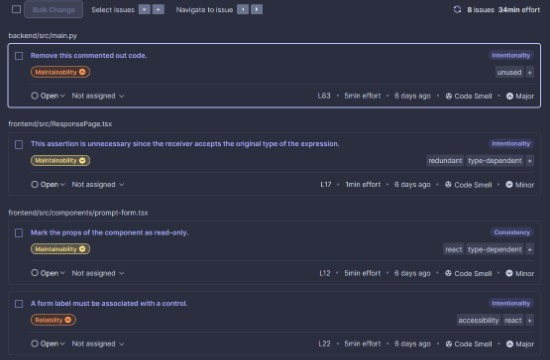
\includegraphics[width=1\linewidth]{Image5.jpg}
    \caption{Maintainability issues in the codebase.}
    \label{fig:figure7}
\end{figure}

The maintainability issues require a systematic solution involving large-scale refactoring. Commented code must be removed entirely rather than being left as useless baggage in the codebase. Addition of proper accessibility features to user interface elements would increase usability and fulfill the requirements of modern web standards. Refactoring the frontend framework would allow for the reduction of coupling between components, thus increasing modularity and testability. Proper documentation for complex parts of the code would help in future maintenance efforts.

\begin{figure}[htbp]
    \centering
    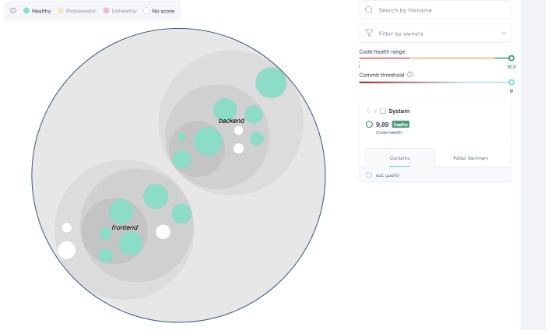
\includegraphics[width=1\linewidth]{Image6.jpg}
    \caption{Code health overview.}
    \label{fig:figure8}
\end{figure}

\subsection{Architectural Assessment}
The backend structure (see Figure \ref{fig:figure1}) of the system is modular with several separate parts, like the entry point for the FastAPI application, the message and response routers for handling requests, the database module for data persistence, the LLM implementation for interaction with the model, and the repository for data. The structure of this design is characterized by many benefits, such as a clear separation of responsibilities across the parts, systematically arranged API endpoints using specialized routers, and a well-defined LLM implementation module for the purpose of handling multiple models.

However, the design leaves potential weaknesses that require further examination. The message\_router appears to be handling all interactions from users, which could be a bottleneck under high loads. The diagrams don't implement full error handling, thus raising the robustness of the system into question. The documentation doesn't separate the authentication and authorization processes, which could be a security weakness. Several components seem to interact with the database directly, which could result in data inconsistency for data manipulation and breaking of the business logic.

Improvements to this architecture should include implementing a service layer between routers and data access components to centralize business logic and ensure consistency. Comprehensive error handling throughout the application would improve reliability and user experience. Considering the potentially resource-intensive nature of LLM requests, implementing a message queue for asynchronous processing would enhance system scalability. Adding security middleware for authentication and authorization would address the identified security concerns.

The frontend architecture (see Figure \ref{fig:figure2}) features React components, with App.tsx serving as the main component, and various components specific to form management and response management, in addition to a shared sidebar component. This setup follows the component-based architecture principles according to React best practices, showing an appropriate separation of concerns between form handling and response display. Nevertheless, the frontend architecture exhibits weaknesses that merit attention. Message handling logic appears duplicated across components, suggesting insufficient abstraction. Form components and state management mechanisms show tight coupling, which complicates testing and reduces reusability. Addressing these issues requires implementing a robust state management solution such as Redux or Context API to centralize application state. Extracting duplicate logic into custom hooks would improve reusability while reducing maintenance overhead. Component composition techniques would enhance UI element reuse across the application.

\subsection{System Health Assessment}
The system health evaluation results in a medium health rating, showing no critical blockers. There are, however, many high-severity issues, with a large number of medium and low-severity issues. The most common focus is on maintainability, with the potential for the accumulation of technological debt across the code.

Addressing these health concerns requires prioritizing high-severity security issues to reduce immediate risk exposure. Implementing comprehensive automated testing would improve reliability scores while providing regression protection during refactoring efforts. Systematically addressing code duplication would enhance maintainability metrics while reducing future maintenance costs. A structured technical debt reduction plan should be developed for the identified issues, with clear prioritization based on risk and business impact.

\subsection{Detailed Security Analysis of LLM Implementation}
The part of the LLM implementation emphasizes specific security aspects relevant for user and system message handling for a variety of LLM implementations. The diagrams don't represent any mechanism for input validation, raising issues on handling user inputs for inputs going into LLMs. Without any such validation, the following is introduced:

Susceptibility for prompt injection attacks that could change the behavior of the LLM, malformed JSON possibly leading to application faults, as well as resource exhaustion from large inputs. To mitigate these risks, it is critical to implement strict JSON schema validation of incoming data, institute appropriate input size limits and content filtering mechanisms, rate limiting on API interfaces, and consider the possible addition of a dedicated prompt security framework to prevent prompt injection attacks. The institution of these controls would significantly improve the security posture of the components handling LLM interactions.

The diagrams contain no obvious authentication and authorization mechanisms, which is of concern for the application that is being used for sending possibly sensitive communications with LLMs. Incorporating OAuth 2.0, or API key authentication, would allow for the authentication of users. Role-based access control would allow for varied permissions among disparate user groups. In-depth logging and auditing of any message submissions and resultant replies would increase security surveillance and meet compliance requirements. Separate access controls for a variety of LLM models would allow for a sophisticated level of security customized for disparate sensitivity levels.

The database operations provide limited information regarding data encryption and the relevant security measures. Encryption of sensitive data retained in the system is a key security feature relevant to this category of applications. Database access controls should restrict data visibility according to defined need-to-know factors. Considering the nature of interactions involved with the LLM, applying anonymization or tokenization of user inputs, where possible, would reduce privacy risks. Proper data retention procedures would enable compliance with privacy laws while also minimizing the propagation of unnecessary information.

\subsection{Code Quality Detail Analysis}
The metrics from the software reveal two specific reliability issues from the codebase. The issues most likely reflect exception handling, resource management issues, or concurrency issues that could compromise the reliability of the system. In order to deal with these issues, it is important to implement robust exception handling across the application, implement correct resource deallocation procedures for database connections and file descriptors, implement timeouts for long-running LLM requests, and implement circuit breakers for interactions with other services to prevent cascading failures.

More significantly, the metrics identify six maintainability issues, indicating significant technical debt that can slow down future development velocity. Refactoring duplicated code into shared utility methods would improve maintainability and reduce the risks that come with inconsistencies. Comprehensive documentation would make knowledge transfer and maintenance easier. The implementation of consistent coding standards throughout the application would improve readability and maintainability. Overly complex components should be incrementally refactored to enhance their structure without altering functionality.

\section{Implementation Recommendations}
From this in-depth analysis, several priorities of implementation are evident. The most important is seen to be the improvement of security, calling for remedial action on container security through proper user permissions, the use of HTTPS throughout the application, proper input validation and sanitization practices, and secure file handling practices. These changes would effectively address the most critical vulnerabilities identified in the analysis.

Code quality improvements are the second priority area, which include refactoring duplicated message handling functions, removing commented-out code and outdated code blocks, fixing accessibility issues in the user interface, and implementing comprehensive error handling mechanisms. These improvements are expected to reduce technical debt while at the same time improving maintainability and reliability. Architectural enhancements form the tertiary priority area, including the addition of a service layer between data access modules and API endpoints, the creation of overall state management for the frontend, the consideration of asynchronous processing for LLM requests, and the addition of monitoring and observability features. These changes are expected to increase the scalability, reliability, and maintainability of the system over time.

\section{Limitations and Future Work}
\subsection{Limitations of the Assessment}
Our quality assessment had several limitations:
\begin{itemize}
\item Limited performance testing under high load conditions
\item Incomplete analysis of authentication and authorization mechanisms
\item Focus primarily on code quality rather than user experience
\item Limited comparison with similar systems or industry benchmarks
\end{itemize}

\subsection{Future Work}
Future work should include:
\begin{itemize}
\item Implementing the recommended security improvements as highest priority
\item Developing a comprehensive refactoring plan to address code duplication
\item Enhancing the architecture with service layers and improved state management
\item Implementing continuous monitoring for ongoing quality assessment
\item Conducting thorough security testing, including penetration testing
\end{itemize}

\section{Conclusion}
The LLM Message Dispatch Tool shows promise via its modular architecture and clear component separation; however, it requires significant attention to security vulnerabilities and code quality issues. The identified security vulnerabilities surrounding privileged container running, insecure file transfer, and unencrypted data communication represent actual risks that require immediate remediation. Additionally, the issues with code quality in the areas of redundancy and maintainability indicate technical debt accumulation that will impede future development if not systematically addressed.

The architectural assessment reveals both strengths and opportunities for improvement in both front-end and backend components. Implementing a service layer, improving state management, and enhancing security controls would significantly improve the system's resilience, maintainability, and security posture. The system health assessment indicates moderate overall health with specific focus areas requiring attention.

Resolution of these matters with the top-down implementation approach would make the application more dependable, manageable, and secure, thus better enabling the critical operation of sending messages to other implementations of the LLM. The proposals listed here serve as the basis for such development, well-matching pressing security issues with future improvements in code and design.

\bibliography{references}
\appendix

\end{document}